\chapter{Anhang}

\begin{figure}[htbp]
    \centering
    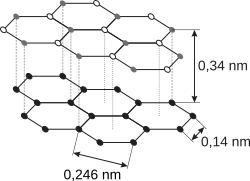
\includegraphics[width=0.75\textwidth]{figs/HOPG_struktur.png}
    \caption{Zwei übereinander gestapelte Schichten von Graphit (HOPG), die die hexagonale Anordnung der Kohlenstoffatome zeigen. Schwarze Punkte markieren Atome, die direkt über einem Atom in der darunterliegenden Schicht sitzen, weiße Punkte solche, die dies nicht tun. Die C–C-Bindung in der Ebene beträgt \SI{0.14}{\nano\metre}, die Gitterkonstante ist \SI{0.246}{\nano\metre} und der Schichtabstand beträgt \SI{0.34}{\nano\metre}.  \cite{praktikum}}
    \label{fig:HOPG struktur}
\end{figure}

\begin{figure}[htbp]
    \centering
    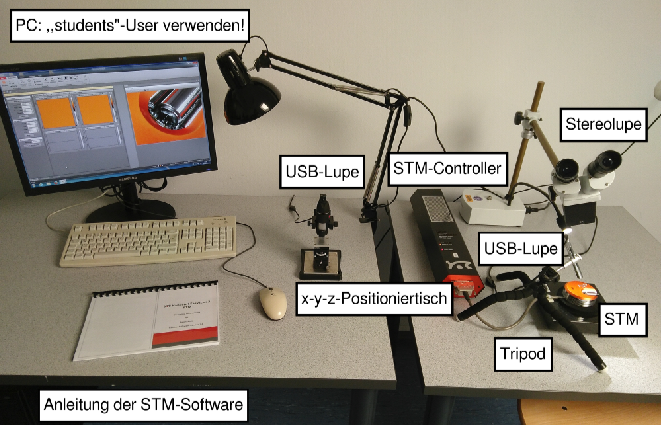
\includegraphics[width=0.75\textwidth]{figs/Versuchsaufbau1.png}
    \caption{Experimentelle Station für das P422-Rastertunnelmikroskopie-Experiment. \cite{praktikum}}
    \label{fig:Versuchaufbau1}    
\end{figure}

\begin{figure}
    \centering
    \includegraphics[width=0.75\textwidth]{figs/Versuch_box}
    \caption{Weitere Materialien für den Aufbau. \cite{praktikum}}
    \label{fig:Versuch box}
\end{figure}